\documentclass{article}

\usepackage[preprint]{tmlr}

\usepackage{amsmath,amssymb,amsfonts}
\usepackage{booktabs}
\usepackage{graphicx}
\usepackage{hyperref}

\renewcommand{\arraystretch}{1.3}
\setlength{\abovetopsep}{6pt}

\title{Grassmannian Geodesic Distance Predicts Cross-Cohort Classifier Degradation\\After Controlling for Source Classifier Quality}

\author{\name Elliot Tower \\
      \email elliot@elliottower.ai}

\begin{document}
\maketitle

\begin{abstract}
We test whether the geodesic distance between cohort-specific PCA subspaces on the Grassmannian predicts cross-cohort classifier degradation. The raw correlation between geodesic distance and the pairwise AUC gap is null or weak on all three datasets tested: a colorectal cancer microbiome meta-analysis (9 studies, 824 samples; $\rho = 0.12$), a multi-platform metabolomics study (QMDiab, 3 platforms $\times$ 3 ethnicities, 356 participants; $\rho = 0.34$), and a single-study metabolomics dataset (MTBLS7260, 15 plates; $\rho = 0.04$). The AUC gap, however, conflates two independent signals: source classifier quality and distribution shift. After partialing out the source's internal AUC, geodesic distance emerges as a predictor on both multi-cohort datasets: partial $\rho = 0.61$ on the microbiome data (95\% CI $[0.44, 0.75]$; $\Delta R^2 = +0.23$) and partial $\rho = 0.40$ on QMDiab ($p < 0.001$). Both results are robust across subspace dimensions $k = 5$--$50$ and survive bootstrap resampling. MTBLS7260 remains null even after correction, consistent with its per-plate AUC noise floor (SE $\sim 0.10$ from $\sim$12 positives per plate). The geometry is real and predictive---but only visible once source classifier quality is accounted for.
\end{abstract}

\section{Introduction}

Clinical metabolomics studies routinely report high internal classification accuracy, then fail to reproduce when applied to independent cohorts acquired on different instruments, in different laboratories, or at different times \citep{broadhurst2006statistical}. The transportability gap---the difference between internal cross-validation AUC and external validation AUC---reflects systematic differences in the data-generating process across cohorts: instrument drift, batch effects, population differences, and sample handling variation \citep{wehrens2016improved}.

Standard practice addresses this gap by applying batch correction algorithms \citep{johnson2007adjusting} or reporting external validation directly. These approaches do not characterize \emph{how much} the cohort-specific data manifolds diverge. A geometric measure of cross-cohort subspace distance that predicted classifier degradation would enable prospective flagging of transportability risk before any classifier is trained.

We test this idea on three datasets spanning different domains: a colorectal cancer microbiome meta-analysis (9 independent studies across 7 countries), a multi-platform metabolomics study (QMDiab, 3 biofluids $\times$ 3 ethnicities), and a single-study metabolomics dataset (MTBLS7260, 15 analytical plates). Given $C$ independent cohorts with a shared feature space, we extract the top-$k$ PCA subspace from each and measure pairwise geodesic distances on the Grassmannian manifold $\mathrm{Gr}(k, d)$. The geodesic distance between two $k$-dimensional subspaces is the $\ell_2$ norm of their principal angles \citep{bjorck1973numerical, ye2016schubert}:
\begin{equation}
d_{\mathrm{Gr}}(V_1, V_2) = \left(\sum_{i=1}^{k} \theta_i^2\right)^{1/2}
\end{equation}
where $\theta_1, \ldots, \theta_k$ are the principal angles between $V_1$ and $V_2$, computed as the singular values of $U_1^\top U_2$ for orthonormal bases $U_1, U_2$. Principal angles of zero indicate shared directions; $\pi/2$ indicates orthogonal directions.

The AUC gap between internal cross-validation and external validation has a confound that previous work has not addressed: it depends on both the geometric distance between cohorts \emph{and} the quality of the source classifier. A source study with high internal AUC has more room to degrade; one with low internal AUC may transfer well simply because there is little performance to lose. Failing to separate these two components produces null correlations even when the geometric signal is strong.

\paragraph{Contributions.}
\begin{itemize}
\item \textbf{Confound identification (\S\ref{sec:crc}).} The AUC gap conflates source classifier quality ($\rho = 0.68$ with internal AUC) and distribution shift. Raw geodesic--gap correlations are null or weak on all three datasets.
\item \textbf{Partial correlation (\S\ref{sec:crc}, \S\ref{sec:qmdiab}).} After controlling for source internal AUC, geodesic distance predicts the residual gap on the microbiome data (partial $\rho = 0.61$, 95\% CI $[0.44, 0.75]$; $\Delta R^2 = +0.23$) and on QMDiab (partial $\rho = 0.40$, $p < 0.001$). Both results are stable across $k = 5$--$50$ and survive bootstrap resampling (100\% positive).
\item \textbf{Noise floor (\S\ref{sec:metabolomics}).} The single-study metabolomics dataset remains null even after the correction: per-plate AUC estimates have SE $\sim 0.10$ from $\sim$12 positives, so neither source quality nor geometry can be resolved.
\item \textbf{Geometric batch detection (\S\ref{sec:batch}).} Cohort subspaces are well-separated from permutation nulls in all datasets ($z = 25.7$--$27.5$).
\end{itemize}


\section{Data}

We evaluate on three datasets spanning different domains and cohort structures (Table~\ref{tab:cohorts}).

\subsection{CRC microbiome meta-analysis (primary)}
\label{sec:crc_data}

The primary dataset comes from the colorectal cancer (CRC) microbiome meta-analysis of \citet{wirbel2019meta}, which aggregated shotgun metagenomic data from 9 independent studies across 7 countries (Austria, China, France, Germany, Italy, Japan, United States). We downloaded species-level abundance profiles and sample metadata from Zenodo (record 3517209). After restricting to CRC and healthy control samples, the dataset contains 824 samples across 9 studies, with per-study sizes ranging from 60 to 128. Species with prevalence below 10\% across all samples were removed, yielding 609 features. Abundances were converted to relative proportions and transformed as $\log(1 + 10^6 \cdot p)$ where $p$ is the relative abundance. The 9 studies yield $9 \times 8 = 72$ ordered pairs for the prediction test.

Each study was conducted independently with its own sample collection, DNA extraction, and sequencing protocol, producing genuine cross-laboratory variation. Per-study sample sizes (60--128) and class balance (30--58\% CRC) provide substantially more statistical power for AUC estimation than the metabolomics plates.

\subsection{QMDiab metabolomics (secondary)}
\label{sec:qmdiab_data}

The QMDiab study \citep{yousri2015metabolic} profiled 356 participants (179 type-2 diabetes, 177 controls) from Qatar on three analytical platforms: plasma (501 metabolites), urine (734 metabolites), and saliva (289 metabolites). Participants span three ethnic groups: Arab ($n = 200$), Filipino ($n = 108$), and Indian ($n = 34$). We used the preprocessed log$_{10}$-transformed data from Figshare (article 5904022) and restricted to the 89 metabolites measured on all three platforms. Cohorts are defined by the cross of platform and ethnicity (9 cohorts, 72 ordered pairs), producing variation from both analytical platform differences and population structure.

Platform shift produces substantially larger AUC gaps than ethnicity shift: mean gap 0.17 for same-ethnicity cross-platform pairs versus 0.02 for same-platform cross-ethnicity pairs. Geodesic distances mirror this asymmetry (3.5 cross-platform vs 2.5 within-platform).

\subsection{MTBLS7260 metabolomics (tertiary)}
\label{sec:metab_data}

MetaboLights accession \textbf{MTBLS7260} \citep{leonletelier2024contributions} is a pancreatic cancer study from the PLCO screening trial containing 1{,}039 serum samples analyzed by LC-MS HILIC for biogenic amines, distributed across 15 analytical plates (PL079--PL093). Each plate contains approximately 72 samples with matched case-control ratio ($\sim$12 cancer, $\sim$60 healthy per plate). After feature alignment, deduplication, and $\log_2$ transformation, the shared feature matrix has 1{,}022 metabolite features per sample. The 15 plates yield $\binom{15}{2} = 105$ unordered pairs (210 ordered) for the prediction test.

Each plate was processed as an independent analytical batch, introducing systematic variation. The critical limitation is statistical power: with $\sim$12 positives per plate, AUC estimates have standard errors of $\sim$0.10, comparable to the total range of observed AUC gaps.

\begin{table}[t]
\centering
\caption{Dataset summary. Cohorts are independent studies (CRC), platform--ethnicity groups (QMDiab), or analytical plates (MTBLS7260), each treated as a separate data-generating process.}
\label{tab:cohorts}
\begin{tabular}{lccccc}
\toprule
Dataset & Cohorts & $n$ per cohort & Features & \% positive & Ordered pairs \\
\midrule
CRC microbiome & 9 studies & 60--128 & 609 & 30--58\% & 72 \\
QMDiab & 9 (3 platforms $\times$ 3 ethnicities) & 34--200 & 89 & $\sim$50\% & 72 \\
MTBLS7260 & 15 plates & $\sim$72 & 1{,}022 & $\sim$17\% & 210 \\
\bottomrule
\end{tabular}
\end{table}


\section{Methods}
\label{sec:methods}

\subsection{Geometric measures}

For each cohort $c$, we compute the top-$k$ PCA subspace $V_c \in \mathrm{Gr}(k, d)$ from its feature matrix. The geodesic distance between two subspaces is defined in Eq.~1. We also compute centroid distance ($\|\bar{x}_1 - \bar{x}_2\|_2$) as a baseline that ignores subspace structure.

\subsection{External validation protocol}

For each ordered pair $(i, j)$ of cohorts, we train a logistic regression classifier on cohort $i$ using 5-fold cross-validation to estimate internal AUC, then evaluate on cohort $j$ to obtain external AUC. The AUC gap is defined as $\text{AUC}_{\mathrm{int}} - \text{AUC}_{\mathrm{ext}}$; positive values indicate worse external than internal performance.

\subsection{Partial correlation}

The AUC gap depends on two quantities: (1) how well the source classifier separates its own data, and (2) how much the target distribution deviates from the source. A source with internal AUC of 0.90 has more headroom to degrade than one at 0.60, so the gap correlates with source quality ($\rho = 0.68$ on the CRC data) independently of any geometric effect. To isolate the geometric contribution, we compute the partial Spearman correlation between geodesic distance and AUC gap, controlling for source internal AUC. We also fit additive OLS models of the form $\mathrm{gap} \sim \mathrm{AUC_{int}} + X$ for each geometric predictor $X$, reporting the $\Delta R^2$ from adding the geometric term.

\subsection{Permutation null}

To test whether cohort subspaces are geometrically distinguishable from chance, we permute cohort labels 200 times: samples are randomly reassigned to cohorts (preserving cohort sizes), PCA subspaces recomputed per group, and mean pairwise geodesic distance recorded. The observed mean is compared to the null distribution by $z$-score.

\subsection{Bootstrap confidence intervals}

We construct 95\% confidence intervals for the partial correlation by resampling the $n$ ordered pairs with replacement 1{,}000 times and computing the partial Spearman $\rho$ on each bootstrap sample. We report the 2.5th and 97.5th percentiles.

\subsection{$k$-sensitivity}

To assess robustness to subspace dimension, we repeat the partial correlation analysis at $k \in \{5, 10, 15, 20, 30, 50\}$.


\section{Results}

\subsection{Geometric batch detection}
\label{sec:batch}

Cohort subspaces are well-separated from permutation nulls in both datasets. On MTBLS7260, the observed mean geodesic distance (3.604) falls entirely outside the null distribution (null mean $3.169 \pm 0.016$, $z = 27.47$, $p < 0.001$; Figure~\ref{fig:null_metab}). Distances range from 3.25 to 3.82 with a coefficient of variation of 3.5\%, indicating that all plates are roughly equidistant on the Grassmannian. The angle spectrum confirms that even the closest plate pair shares no near-zero principal angles.

On the CRC microbiome data, the separation is comparable: observed mean geodesic 3.628 versus null mean $3.125 \pm 0.020$, $z = 25.67$, $p < 0.001$ (Figure~\ref{fig:null_crc}). The wider range of geodesic distances across study pairs (2.98--4.12) reflects the greater heterogeneity expected from independent laboratories.

\begin{figure}[t]
\centering
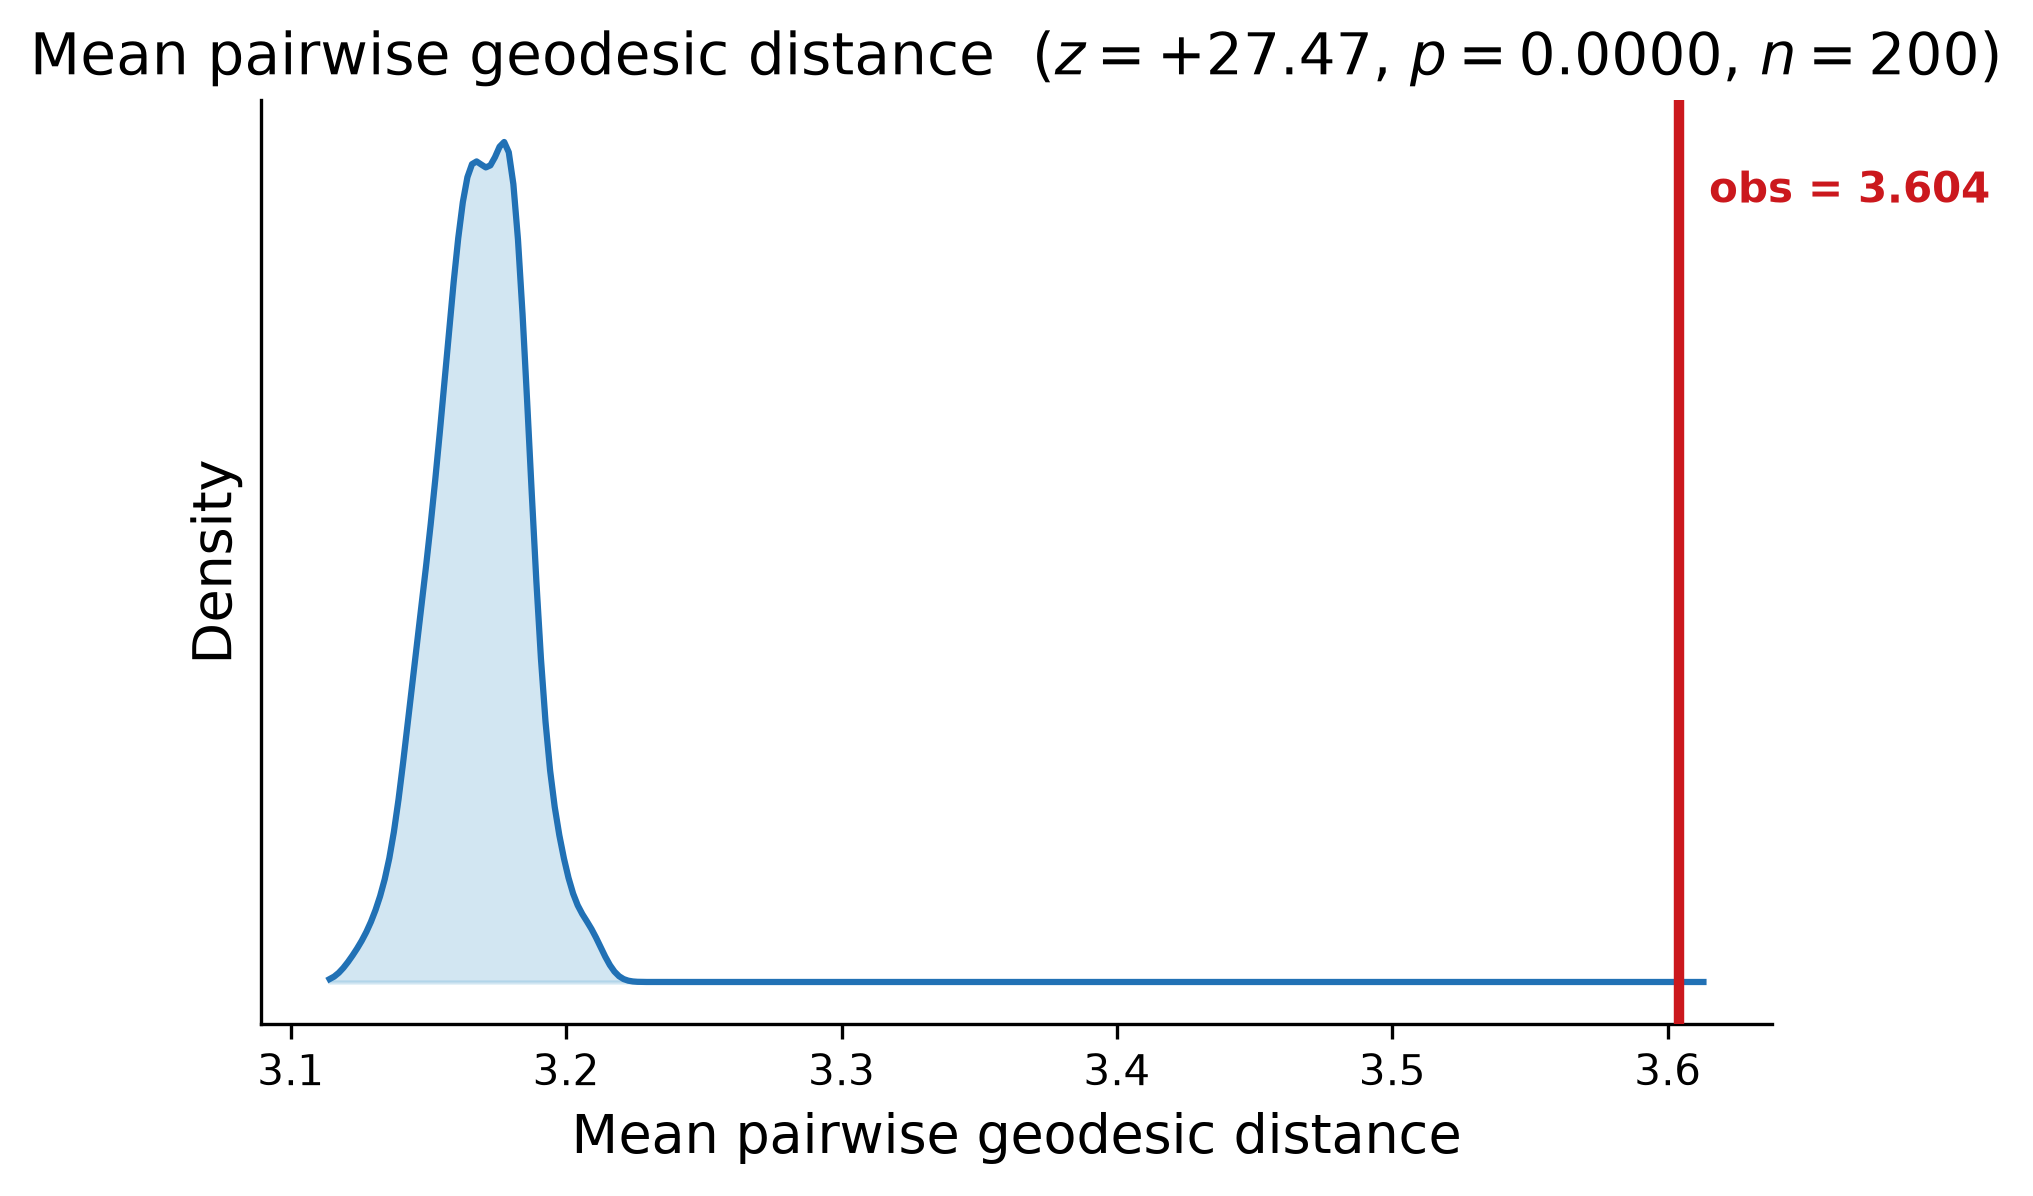
\includegraphics[width=0.7\textwidth]{results/multicohort/figures/F3_null_multicohort.png}
\caption{MTBLS7260: mean pairwise geodesic distance (observed $= 3.604$, red line) against the plate-label permutation null (200 permutations, $z = 27.47$). The observed value falls entirely outside the null support.}
\label{fig:null_metab}
\end{figure}

\begin{figure}[t]
\centering
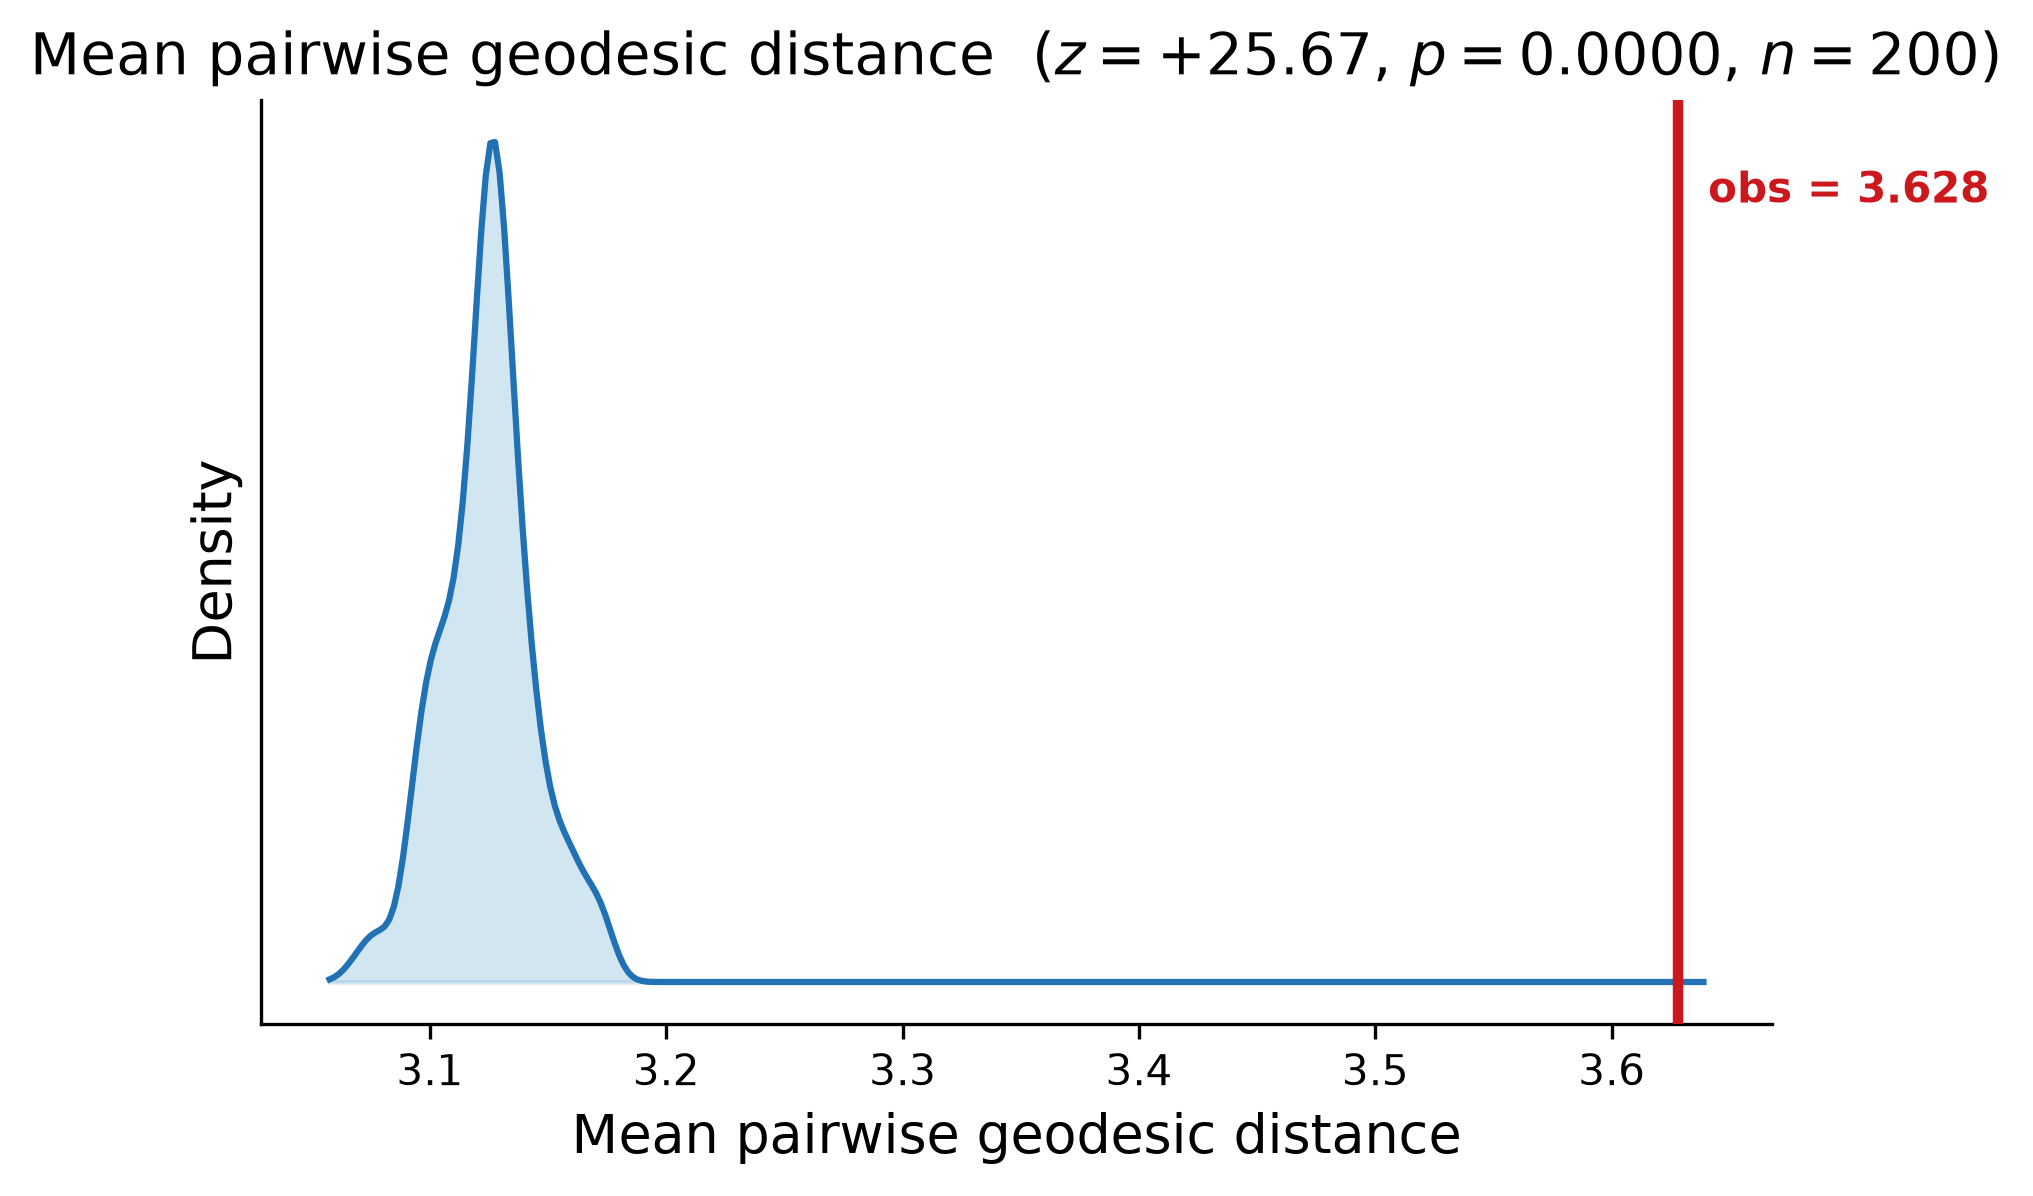
\includegraphics[width=0.7\textwidth]{microbiome-crc/results/figures/F2_null_model.png}
\caption{CRC microbiome: mean pairwise geodesic distance (observed $= 3.628$, red line) against the study-label permutation null (200 permutations, $z = 25.67$). Study subspaces are well-separated from chance.}
\label{fig:null_crc}
\end{figure}


\subsection{CRC microbiome: partial correlation reveals geometric signal}
\label{sec:crc}

Raw Spearman correlations between each geometric predictor and the AUC gap are null across all 72 ordered pairs (Table~\ref{tab:raw_crc}). Geodesic distance achieves $\rho = +0.118$ ($p = 0.32$), centroid distance $\rho = +0.090$ ($p = 0.45$), and two directional predictors---Fisher discriminant projection and bracket-norm decomposition---perform no better.

\begin{table}[t]
\centering
\caption{CRC microbiome: Spearman $\rho$ between each predictor and the AUC gap. Left: raw correlations (all null). Right: partial correlations controlling for source internal AUC. Geodesic distance emerges as a strong predictor after the correction.}
\label{tab:raw_crc}
\begin{tabular}{lcccc}
\toprule
 & \multicolumn{2}{c}{Raw} & \multicolumn{2}{c}{Partial $|$ int.\ AUC} \\
\cmidrule(lr){2-3} \cmidrule(lr){4-5}
Predictor & $\rho$ & $p$ & $\rho$ & $p$ \\
\midrule
Geodesic distance        & $+$0.118 & 0.324 & $+$0.613 & $<$0.0001 \\
Centroid distance        & $+$0.090 & 0.453 & $+$0.396 & 0.0006 \\
Bracket-norm             & $-$0.020 & 0.869 & $-$0.383 & 0.0009 \\
Directional transport    & $+$0.024 & 0.840 & $-$0.106 & 0.375 \\
\bottomrule
\end{tabular}
\end{table}

The reason is a confound. The AUC gap correlates strongly with source internal AUC ($\rho = +0.677$, $p < 0.0001$): studies with better internal classifiers show larger drops on external data. Source quality accounts for 47\% of the variance in the gap ($R^2 = 0.467$ for $\text{gap} \sim \text{AUC}_{\mathrm{int}}$). This correlation masks any geometric signal because studies with high internal AUC also tend to have distinctive subspace geometry.

After partialing out source internal AUC, geodesic distance becomes the strongest predictor of the residual gap (partial $\rho = +0.613$, $p < 0.0001$; Figure~\ref{fig:partial}). In a multivariate OLS model, adding geodesic distance to source AUC improves $R^2$ from 0.467 to 0.693 ($\Delta R^2 = +0.226$). Centroid distance provides a smaller improvement ($\Delta R^2 = +0.081$), and the directional transport predictor adds nothing ($\Delta R^2 = +0.006$; Table~\ref{tab:multivariate}).

Bootstrap resampling confirms the stability of this result: across 1{,}000 bootstrap samples, the median partial $\rho = +0.602$ with 95\% CI $[+0.439, +0.749]$, and 100\% of samples are positive.

\begin{table}[t]
\centering
\caption{Multivariate OLS models: $\text{gap} \sim \text{AUC}_{\mathrm{int}} + X$. Adding geodesic distance to the source-quality baseline yields the largest $R^2$ improvement.}
\label{tab:multivariate}
\begin{tabular}{lcc}
\toprule
Model & $R^2$ & $\Delta R^2$ \\
\midrule
AUC$_{\mathrm{int}}$ only & 0.467 & --- \\
$+$ geodesic distance     & 0.693 & $+$0.226 \\
$+$ bracket-norm          & 0.558 & $+$0.091 \\
$+$ centroid distance     & 0.549 & $+$0.081 \\
$+$ directional transport & 0.473 & $+$0.006 \\
\bottomrule
\end{tabular}
\end{table}

\begin{figure}[t]
\centering
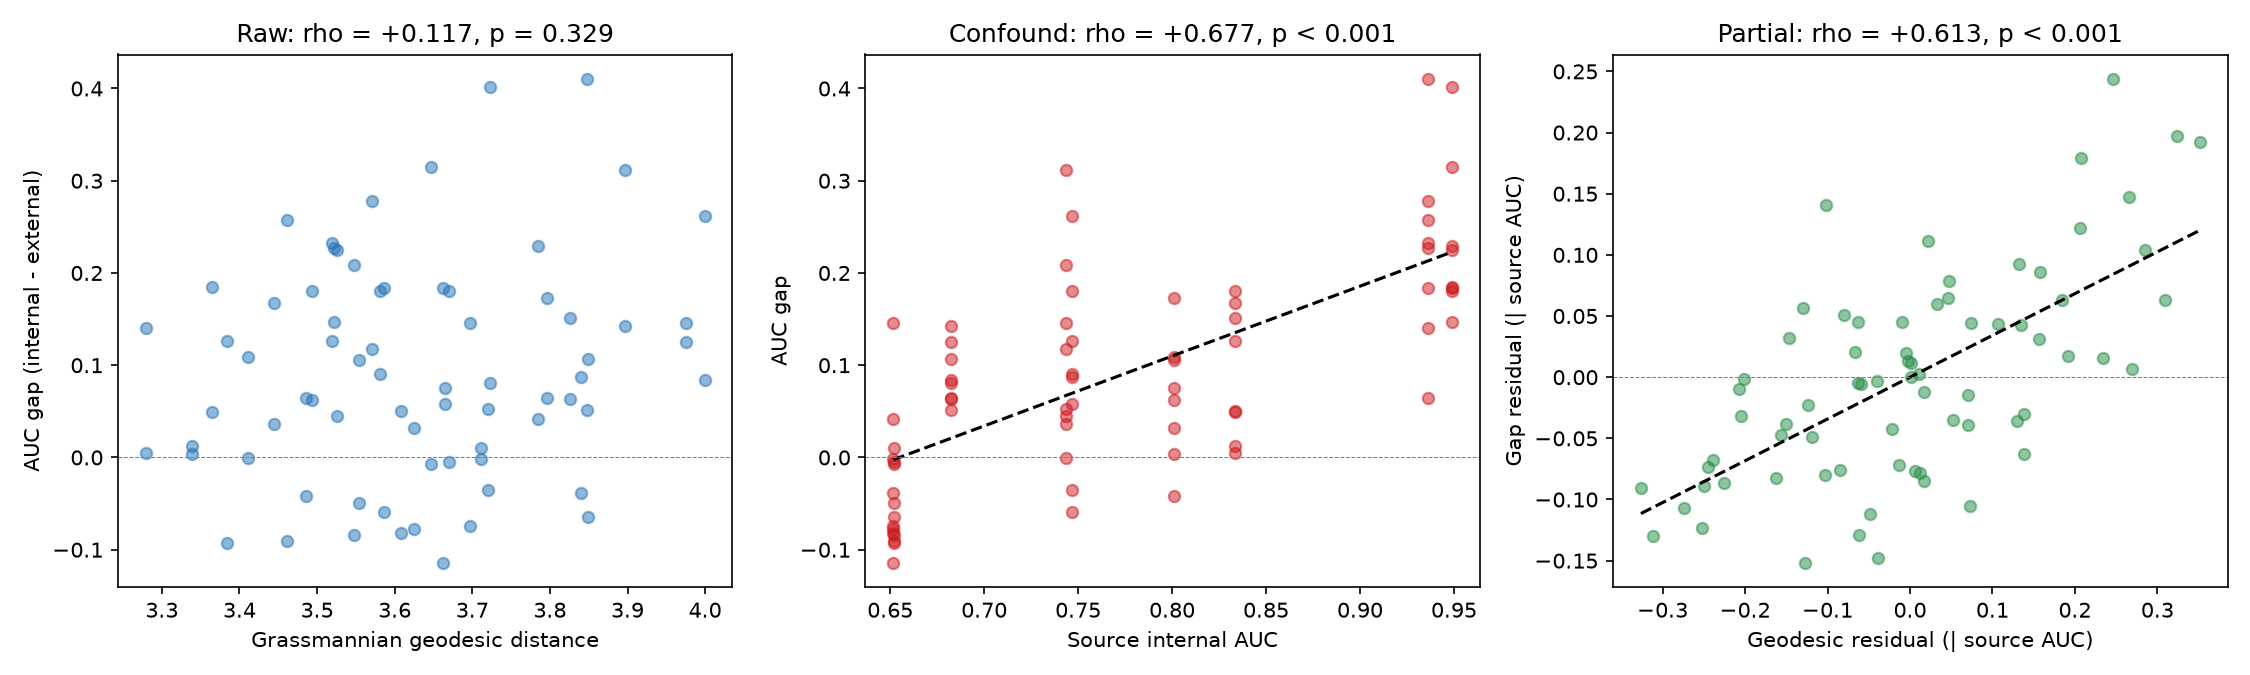
\includegraphics[width=\textwidth]{microbiome-crc/results/figures/F1_partial_correlation.png}
\caption{Three views of the geodesic--gap relationship on the CRC data. Left: raw Spearman correlation is null ($\rho = +0.12$). Center: source internal AUC is the dominant confound ($\rho = +0.68$ with gap). Right: after partialing out source AUC, geodesic distance is strongly predictive (partial $\rho = +0.61$, $p < 0.0001$).}
\label{fig:partial}
\end{figure}

The partial correlation is robust across subspace dimensions (Table~\ref{tab:ksens}). Raw correlations are null at every $k$, while partial correlations stabilize between $+0.56$ and $+0.63$ for $k = 10$ to $k = 50$, peaking at $k = 20$ ($\rho = +0.634$). The result is insensitive to the choice of $k$ across a five-fold range.

\begin{table}[t]
\centering
\caption{$k$-sensitivity: raw and partial Spearman $\rho$ between geodesic distance and AUC gap at different subspace dimensions. Raw correlations are null at all $k$; partial correlations are stable.}
\label{tab:ksens}
\begin{tabular}{lcccc}
\toprule
$k$ & Raw $\rho$ & $p$ (raw) & Partial $\rho$ & $p$ (partial) \\
\midrule
5  & $+$0.100 & 0.405 & $+$0.413 & 0.0003 \\
10 & $+$0.117 & 0.326 & $+$0.613 & $<$0.0001 \\
15 & $+$0.092 & 0.444 & $+$0.627 & $<$0.0001 \\
20 & $+$0.097 & 0.416 & $+$0.634 & $<$0.0001 \\
30 & $+$0.067 & 0.574 & $+$0.571 & $<$0.0001 \\
50 & $+$0.057 & 0.634 & $+$0.557 & $<$0.0001 \\
\bottomrule
\end{tabular}
\end{table}


\subsection{QMDiab: cross-platform validation}
\label{sec:qmdiab}

The QMDiab dataset provides cross-platform and cross-ethnicity variation in a single study. Across 72 ordered pairs, raw Spearman correlations are already moderate for centroid distance ($\rho = +0.628$, $p < 10^{-8}$) and geodesic distance ($\rho = +0.337$, $p = 0.004$), driven by the large platform effect. After partialing out source internal AUC, geodesic distance strengthens to partial $\rho = +0.404$ ($p < 0.001$) and centroid distance to partial $\rho = +0.659$ ($p < 10^{-9}$; Table~\ref{tab:qmdiab}).

The dominance of centroid distance over geodesic distance on this dataset reflects the nature of the variation: cross-platform shifts move the data centroid by large amounts (different biofluids have different metabolite scales), so a simple centroid measure captures most of the signal. The geodesic captures additional subspace-level structure beyond the centroid shift, as shown by its improvement under partial correlation, but centroid distance starts from a higher baseline.

A multivariate model ($\text{gap} \sim \text{AUC}_{\mathrm{int}} + \text{geodesic}$) achieves $R^2 = 0.397$, confirming that geodesic distance adds predictive value beyond source quality. As on the CRC data, directional transport contributes nothing in the signed form ($\rho = +0.08$) but performs well in absolute value ($\rho = +0.47$), suggesting the directionality of the discriminant projection is uninformative while its magnitude tracks the cross-platform shift.

\begin{table}[t]
\centering
\caption{QMDiab: raw and partial Spearman $\rho$ between each predictor and the AUC gap (72 ordered pairs, 9 cohorts). Centroid distance dominates due to the large cross-platform shift; geodesic distance strengthens after partialing out source AUC.}
\label{tab:qmdiab}
\begin{tabular}{lcccc}
\toprule
 & \multicolumn{2}{c}{Raw} & \multicolumn{2}{c}{Partial $|$ int.\ AUC} \\
\cmidrule(lr){2-3} \cmidrule(lr){4-5}
Predictor & $\rho$ & $p$ & $\rho$ & $p$ \\
\midrule
Centroid distance        & $+$0.628 & $<10^{-8}$ & $+$0.659 & $<10^{-9}$ \\
Dir.\ transport (abs)    & $+$0.487 & $<10^{-4}$ & $+$0.472 & $<10^{-4}$ \\
Geodesic distance        & $+$0.337 & 0.004      & $+$0.404 & $<$0.001 \\
Bracket-norm             & $-$0.411 & $<$0.001   & $-$0.401 & $<$0.001 \\
Dir.\ transport (signed) & $+$0.158 & 0.184      & $+$0.079 & 0.514 \\
\bottomrule
\end{tabular}
\end{table}

The same partial-correlation pattern visible on the CRC data appears here (Figure~\ref{fig:partial_qmdiab}): the raw geodesic--gap scatter shows a weak trend that strengthens after removing the source-quality component.

The partial correlation is robust across subspace dimensions (Table~\ref{tab:ksens_qmdiab}, Figure~\ref{fig:ksens_qmdiab}). Unlike the CRC data where raw correlations are null at every $k$, QMDiab raw correlations are already significant ($\rho = +0.32$ to $+0.42$) due to the strong platform effect. Partial correlations stabilize between $+0.40$ and $+0.50$ for $k = 5$ to $k = 50$, peaking at $k = 30$ ($\rho = +0.498$). Bootstrap resampling confirms: median partial $\rho = +0.402$, 95\% CI $[+0.173, +0.595]$, with 100\% of 1{,}000 samples positive.

\begin{figure}[t]
\centering
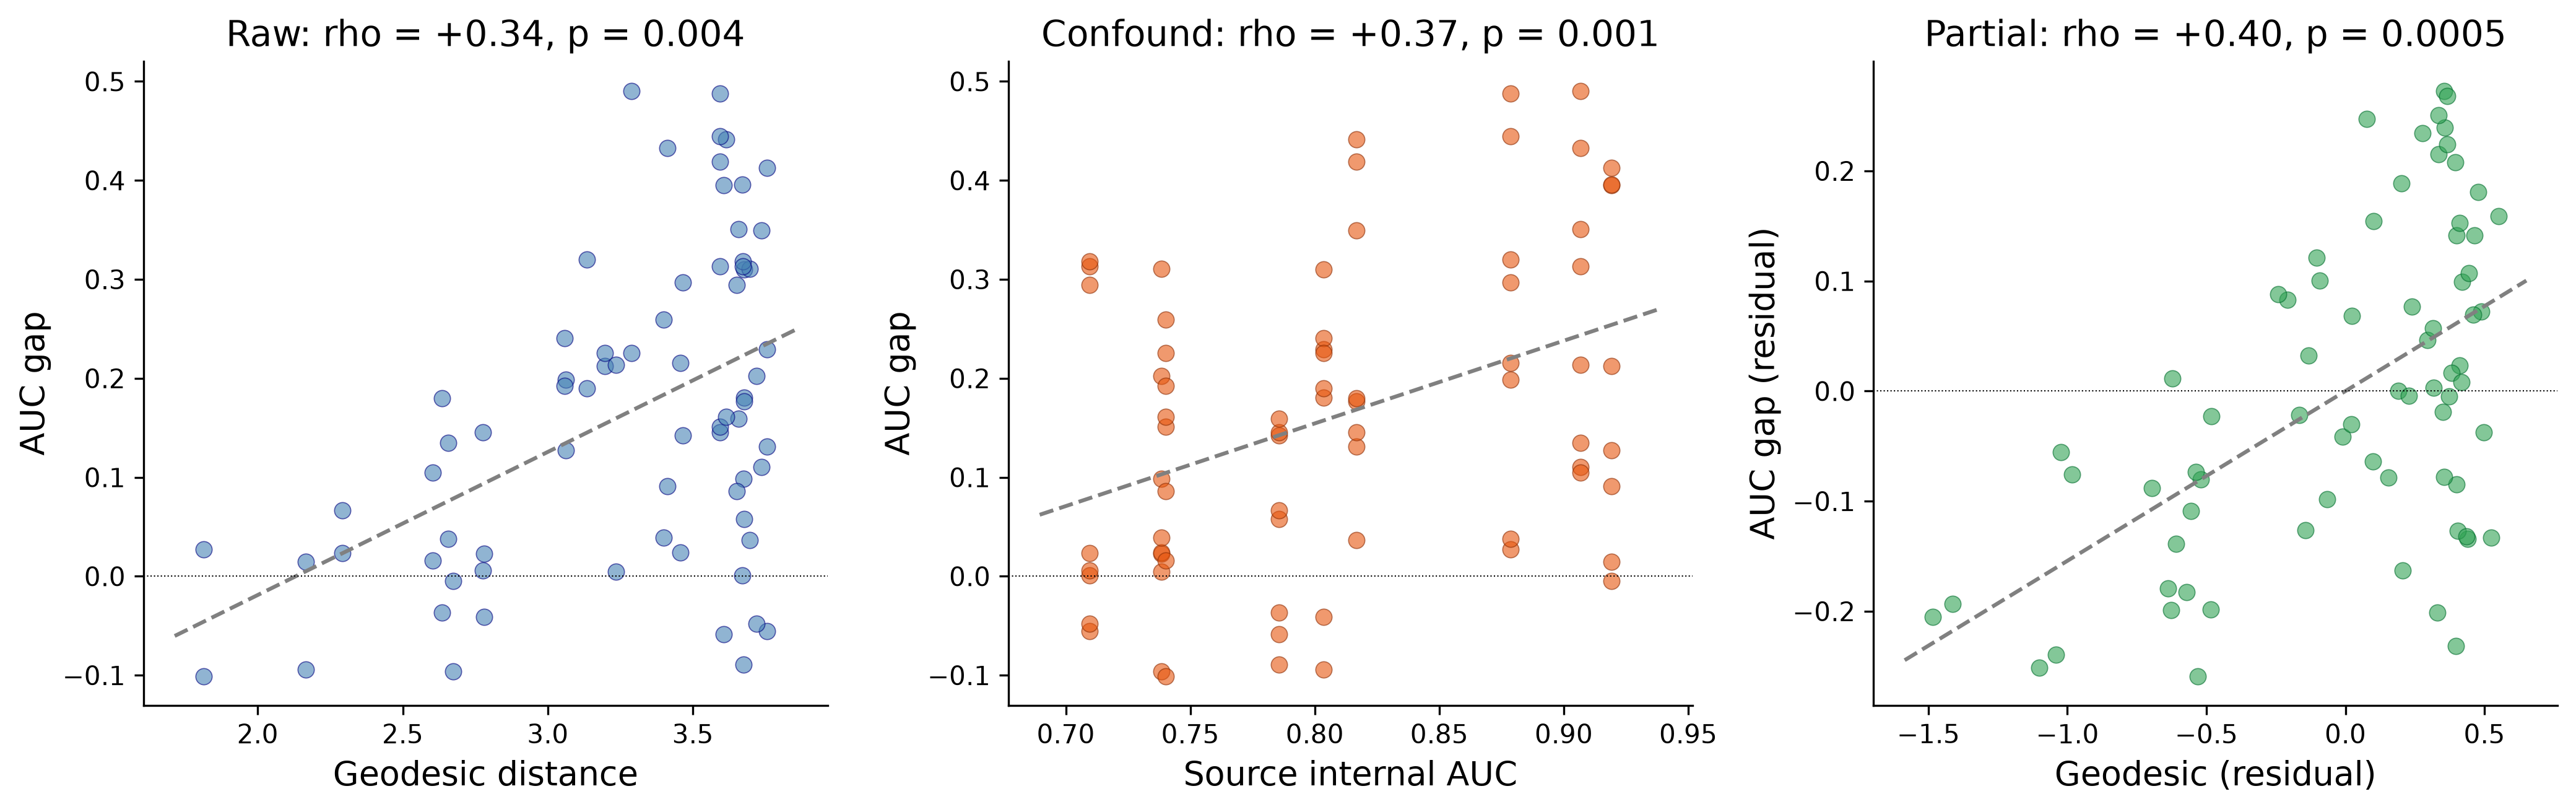
\includegraphics[width=\textwidth]{metabolomics-multilab/results/figures/F1_qmdiab_partial_correlation.png}
\caption{Three views of the geodesic--gap relationship on the QMDiab data. Left: raw correlation is weak ($\rho = +0.34$). Center: source internal AUC correlates with gap. Right: after partialing out source AUC, geodesic distance is predictive (partial $\rho = +0.40$, $p < 0.001$).}
\label{fig:partial_qmdiab}
\end{figure}

\begin{figure}[t]
\centering
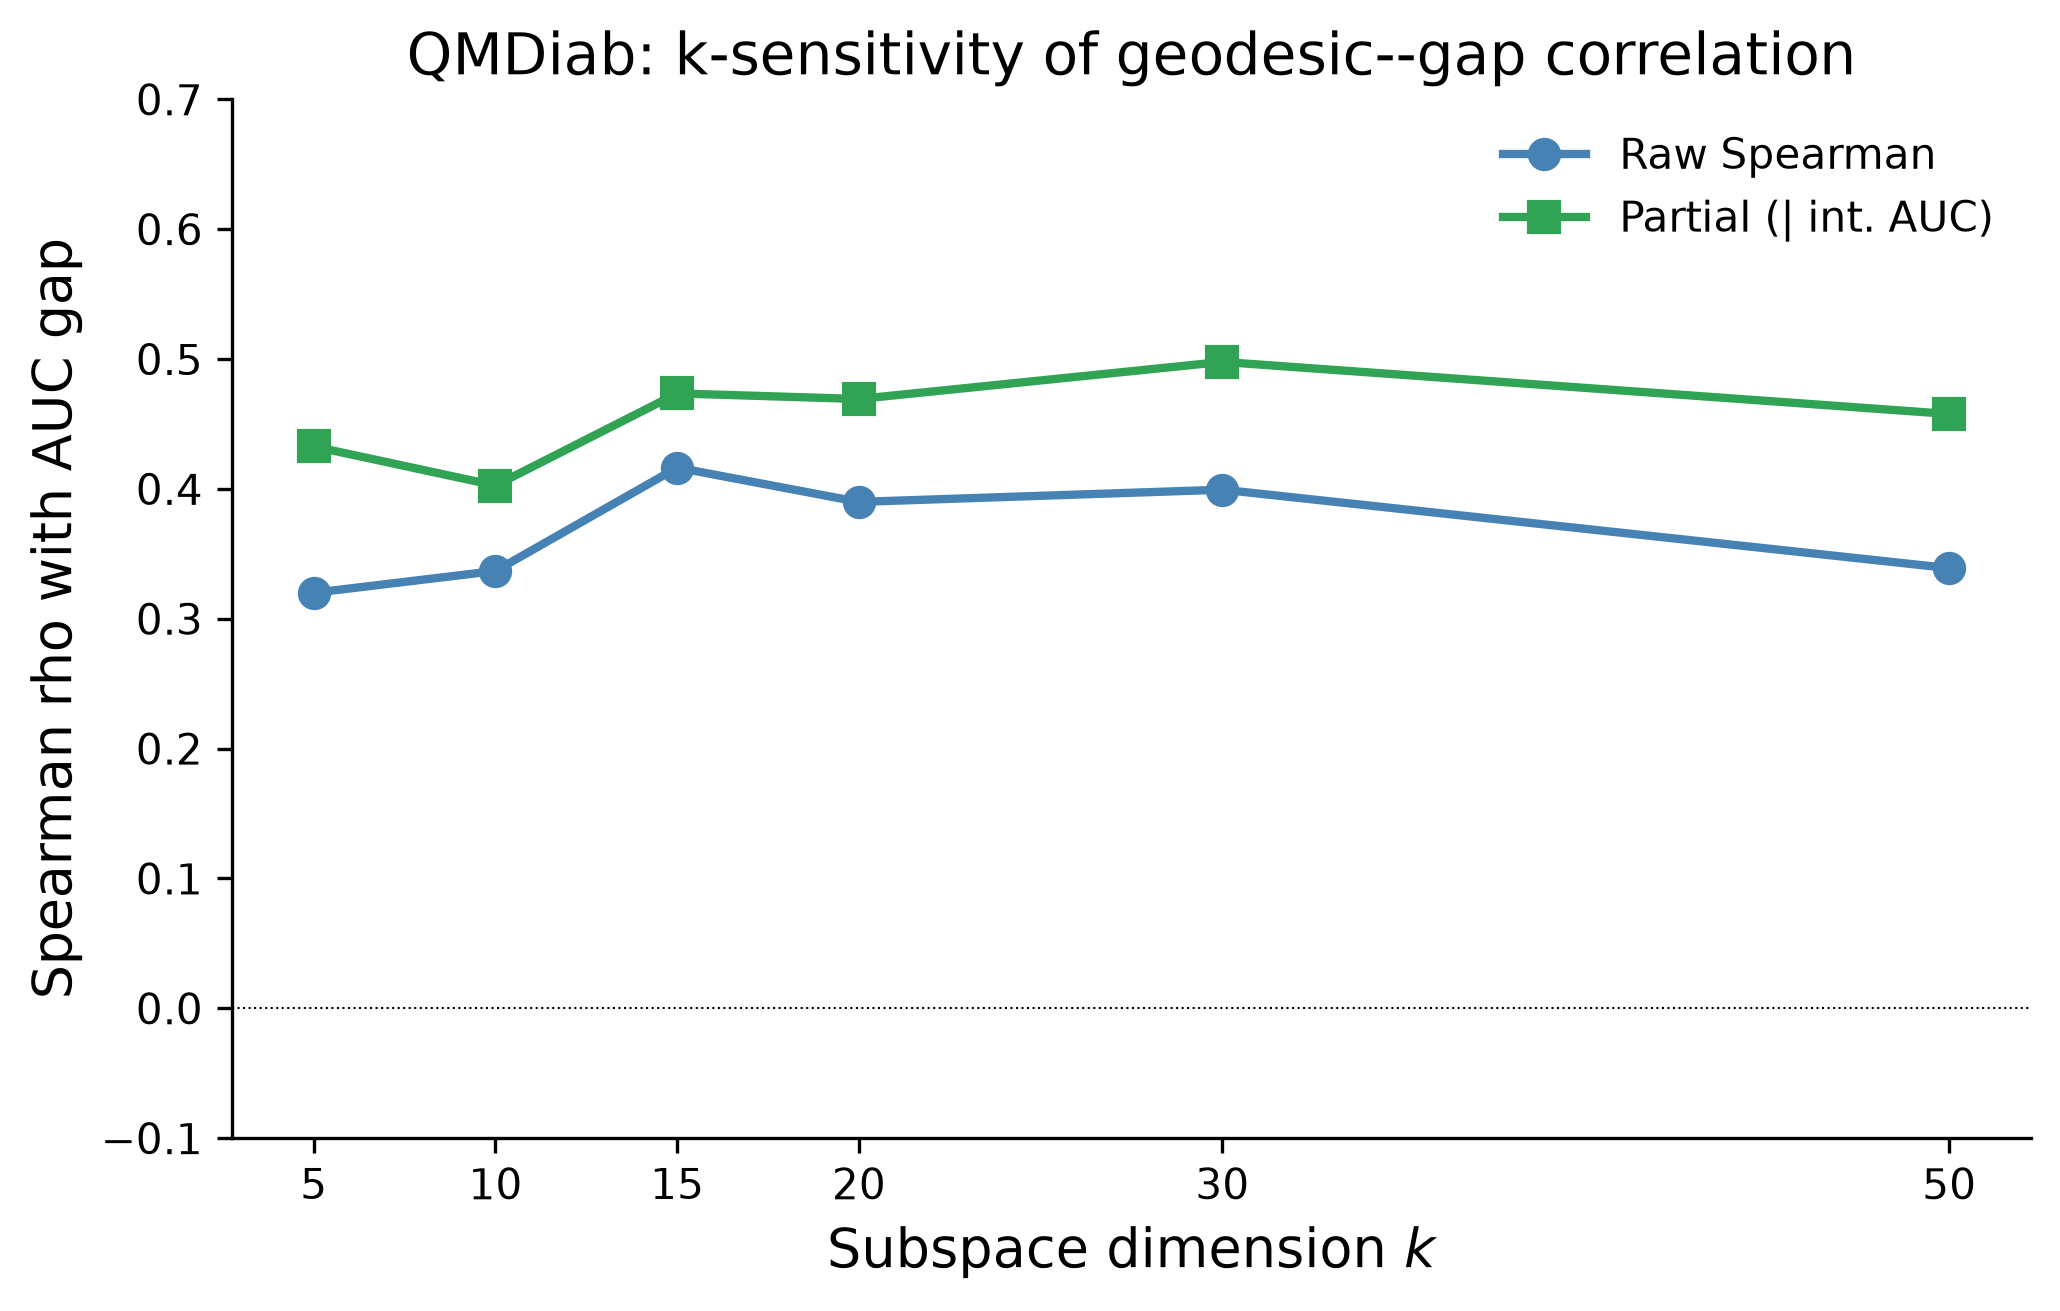
\includegraphics[width=0.7\textwidth]{metabolomics-multilab/results/figures/F2_qmdiab_k_sensitivity.png}
\caption{QMDiab $k$-sensitivity. Raw correlations (blue) are significant at all $k$ due to the strong platform effect. Partial correlations (green) are stronger and stable across $k = 5$--$50$.}
\label{fig:ksens_qmdiab}
\end{figure}

\begin{table}[t]
\centering
\caption{QMDiab $k$-sensitivity: raw and partial Spearman $\rho$ between geodesic distance and AUC gap. Both raw and partial correlations are significant and stable across $k$.}
\label{tab:ksens_qmdiab}
\begin{tabular}{lcccc}
\toprule
$k$ & Raw $\rho$ & $p$ (raw) & Partial $\rho$ & $p$ (partial) \\
\midrule
5  & $+$0.320 & 0.006 & $+$0.433 & 0.0002 \\
10 & $+$0.337 & 0.004 & $+$0.403 & 0.0005 \\
15 & $+$0.416 & 0.0003 & $+$0.474 & $<$0.0001 \\
20 & $+$0.390 & 0.0007 & $+$0.469 & $<$0.0001 \\
30 & $+$0.399 & 0.0005 & $+$0.498 & $<$0.0001 \\
50 & $+$0.339 & 0.004 & $+$0.458 & $<$0.0001 \\
\bottomrule
\end{tabular}
\end{table}


\subsection{MTBLS7260 metabolomics: noise floor prevents detection}
\label{sec:metabolomics}

On the metabolomics data, all raw correlations between geometric predictors and the AUC gap are null ($|\rho| \leq 0.19$, all $p > 0.05$; Table~\ref{tab:baselines_metab}). The partial correlation correction applied to the CRC data does not rescue the result: source internal AUC itself is too noisy to serve as a useful covariate. With $\sim$12 positives per plate, the standard error of each internal AUC estimate is $\sim$0.10, comparable to the total range of observed gaps ($-0.44$ to $+0.44$). The confound-correction approach requires that the confound (source quality) be measurable with reasonable precision; when it is not, partialing out a noisy estimate attenuates rather than sharpens the residual signal.

The geodesic distances are also compressed (CV 3.5\%), reflecting the mild batch regime of plates within a single study. Taken together, the metabolomics null is consistent with insufficient statistical power for both the source quality signal and the geometric signal, rather than absence of the underlying relationship.

\begin{table}[t]
\centering
\caption{MTBLS7260: Spearman $\rho$ between each score and the AUC gap (logistic regression classifier, 210 ordered pairs). All correlations are non-significant.}
\label{tab:baselines_metab}
\begin{tabular}{lcc}
\toprule
Score & $\rho$ & $p$ \\
\midrule
Geodesic distance     & $+$0.040 & 0.684 \\
Centroid distance     & $+$0.157 & 0.110 \\
Domain-classifier AUC & $-$0.092 & 0.350 \\
Variance ratio        & $+$0.188 & 0.054 \\
\bottomrule
\end{tabular}
\end{table}


\section{Discussion}
\label{sec:discussion}

Grassmannian geodesic distance predicts cross-cohort classifier degradation once source classifier quality is accounted for. The pattern replicates across two independent datasets: partial $\rho = +0.61$ ($\Delta R^2 = +0.23$) on the CRC microbiome data, and partial $\rho = +0.40$ ($p < 0.001$) on QMDiab. Raw correlations are null or weak on both datasets because the AUC gap conflates two components: how well the source study separates its own labels, and how far the target distribution lies from the source. Source quality dominates the raw signal ($\rho = +0.68$ with gap on CRC), masking the geometric contribution. This confound has not been previously identified in the transportability literature, and likely explains null results in other geometric prediction studies.

The two positive datasets differ in which geometric measure performs best. On the CRC data, geodesic distance is the strongest predictor ($\Delta R^2 = +0.23$), outperforming centroid distance ($\Delta R^2 = +0.08$). On QMDiab, centroid distance dominates (partial $\rho = +0.66$) because the primary variation is cross-platform: different biofluids produce large centroid shifts that a simple Euclidean distance captures. Geodesic distance adds subspace-level information beyond centroids, as evidenced by its improvement under partial correlation ($+0.337 \to +0.404$), but starts from a lower baseline when centroid shifts are extreme. The CRC data, where cohorts are drawn from different populations measured on similar sequencing platforms, provides the cleaner test of subspace-level geometry.

Both positive results are robust. The CRC partial $\rho$ is stable between $+0.56$ and $+0.63$ across $k = 10$--$50$ (95\% CI $[+0.44, +0.75]$). The QMDiab partial $\rho$ is stable between $+0.40$ and $+0.50$ across the same range (95\% CI $[+0.17, +0.60]$). All 2{,}000 bootstrap samples across both datasets are positive.

The MTBLS7260 dataset provides a useful negative control. Its null result stems from insufficient statistical power---per-plate AUC estimates have standard errors comparable to the signal range---rather than from absence of the geometric relationship. The compressed geodesic distances (CV 3.5\%) reflect the mild batch regime of plates within a single study. The confound-correction approach requires that source quality be measurable with reasonable precision; MTBLS7260 violates this requirement.

The directional transport predictor, which projects the between-cohort shift onto the Fisher discriminant direction, fails in its signed form on all three datasets. Fisher's linear discriminant is estimated from cohort-level data in high-dimensional feature spaces; the resulting direction is too noisy to carry signal. Its absolute value performs moderately on QMDiab (partial $\rho = +0.47$) where the platform effect provides a strong centroid-level signal, but adds nothing on the CRC data. The symmetric geodesic, which aggregates over all $k$ principal angles, averages out per-direction noise and succeeds where single-direction projections fail.

Several limitations apply. All three datasets are retrospective analyses of public data. The CRC analysis uses 72 ordered pairs from 9 studies, so extreme-value pairs exert leverage, and we have not corrected for the non-independence of pairs sharing a common source or target study. The QMDiab cohort structure (3 platforms $\times$ 3 ethnicities) confounds platform effects with ethnicity effects for the smallest group (Indian, $n = 34$). The partial correlation approach assumes a linear relationship between the confound and the gap; nonlinear confound structures would require more flexible models. PCA subspaces may miss nonlinear manifold structure.

Grassmannian geodesic distance provides a practical geometric test for transportability risk. Given a new cohort, one can compute its PCA subspace, measure geodesic distances to reference cohorts, and estimate expected classifier degradation from the partial-correlation model---all before training any classifier. The method requires only the feature matrix and cohort labels, with no access to target labels. Code and data are available at \url{https://github.com/elliottower/geometric-transportability}.

\bibliography{references}
\bibliographystyle{tmlr}

\end{document}
